\section{Simulation results}
In this section, we present the solutions we obtained for the algorithm. To this end, we vary the parameters that affect the simulation. We study five different pairs for the parameters
\begin{equation}
(\Omega, \sigma, x_0) = (1,1,0),\ (1,1,1),\ (1,2,0),\ (2,1,1),\ (2,2,2)	.
\end{equation}
For the spatial discretization, we chose $\Delta = 0.025$ and $L = 1201$. For the discretization in time $\tau = 0.00025$ and $m = 40000$, such that the algorithm stops at $t = m\tau = 10$.
For the positions' averages and variances, we plotted the analytical expectation according to \refEq{eq: x sol} and \refEq{eq: xx sol} in the same plot.
The probability density functions $|\Phi|^2$, are plotted for $t\in [0,2,4,6,8,10]$. {As the Gaussian packet is localized in the vicinity of zero, we chose to plot $x$ from $-5$ to $5$.}
\begin{figure}[h!]
     \begin{subfigure}[h]{1\textwidth}
         \centering
         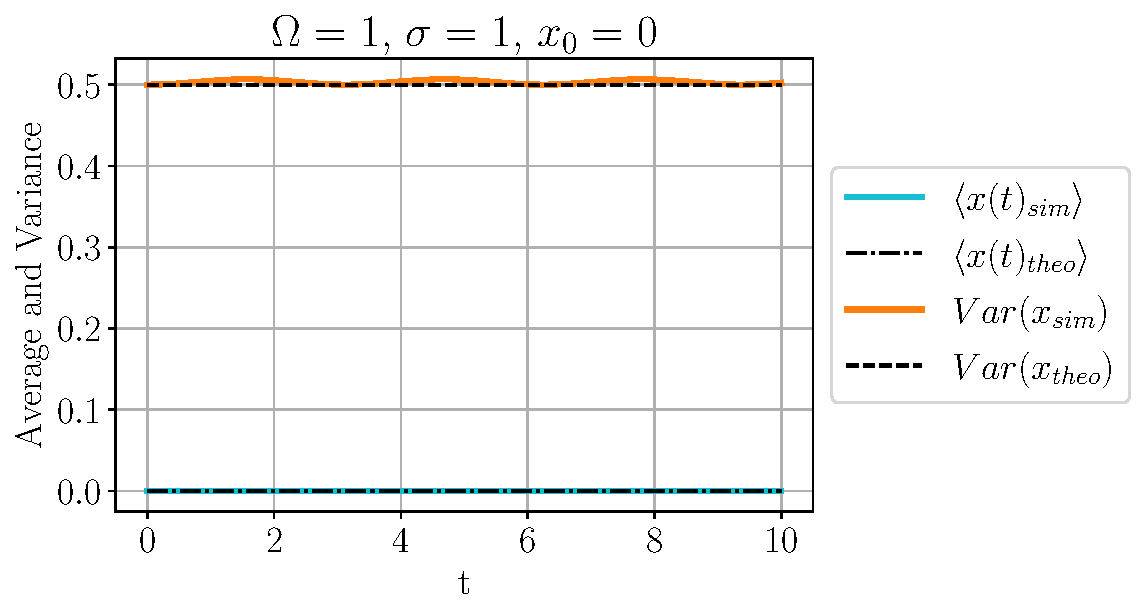
\includegraphics[width=\textwidth]{plot/Omega1_sigma1_x00_Averages.pdf}
         \caption{}
         
     \end{subfigure}
     \begin{subfigure}[h]{1\textwidth}
         \centering
         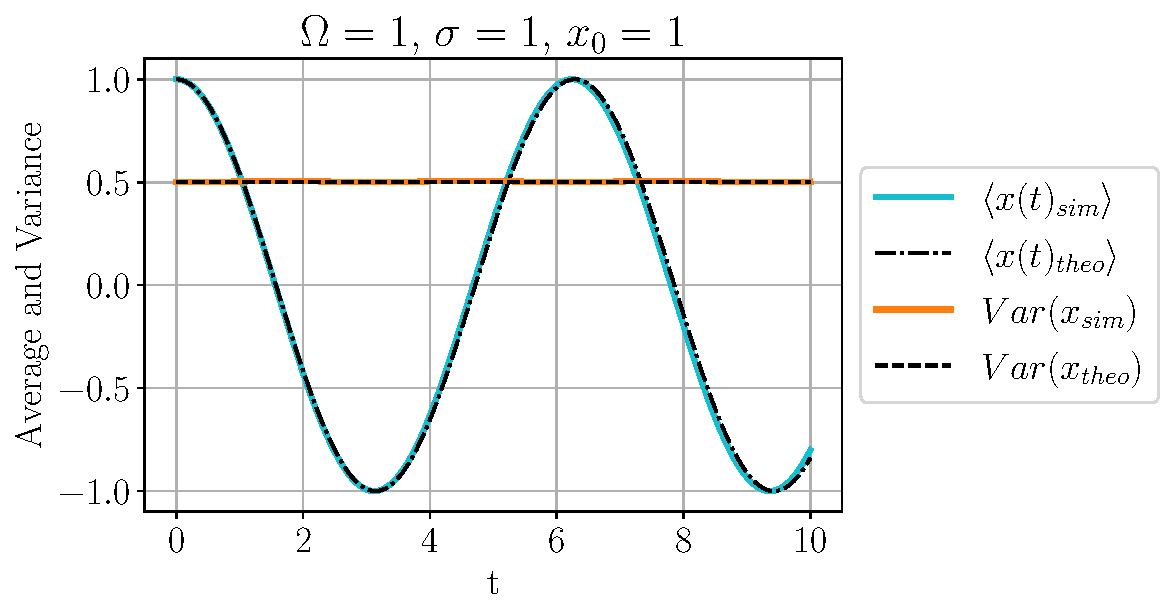
\includegraphics[width=\textwidth]{plot/Omega1_sigma1_x01_Averages.pdf}
         \caption{}
         
     \end{subfigure}
     \begin{subfigure}[h]{0.65\textwidth}
         \centering
         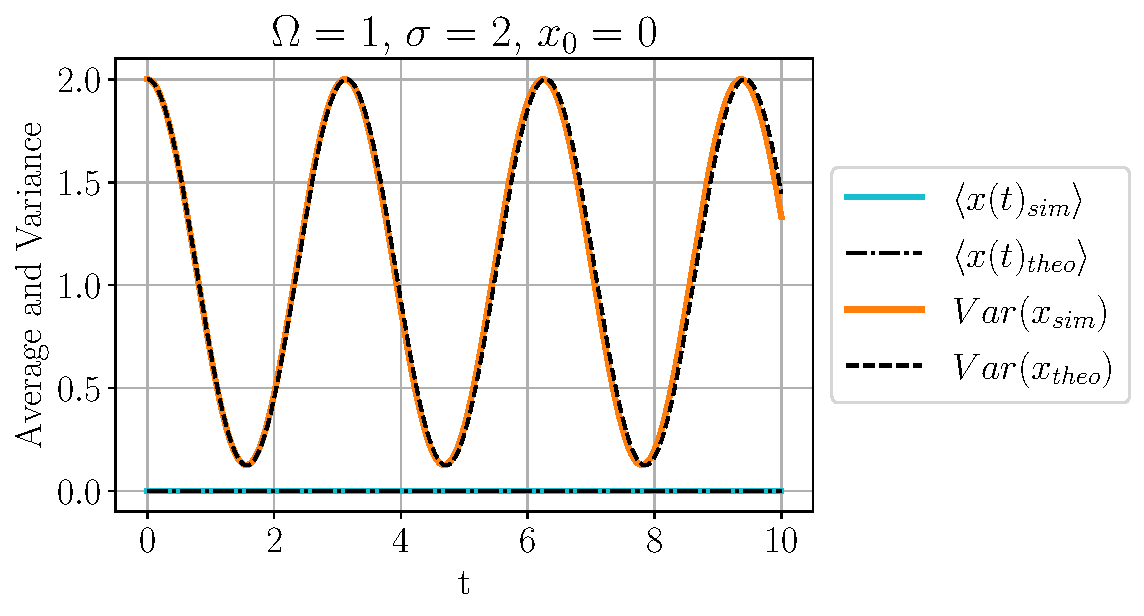
\includegraphics[width=\textwidth]{plot/Omega1_sigma2_x00_Averages.pdf}
         \caption{}
         
     \end{subfigure}
     \begin{subfigure}[h]{0.4\textwidth}
         \centering
         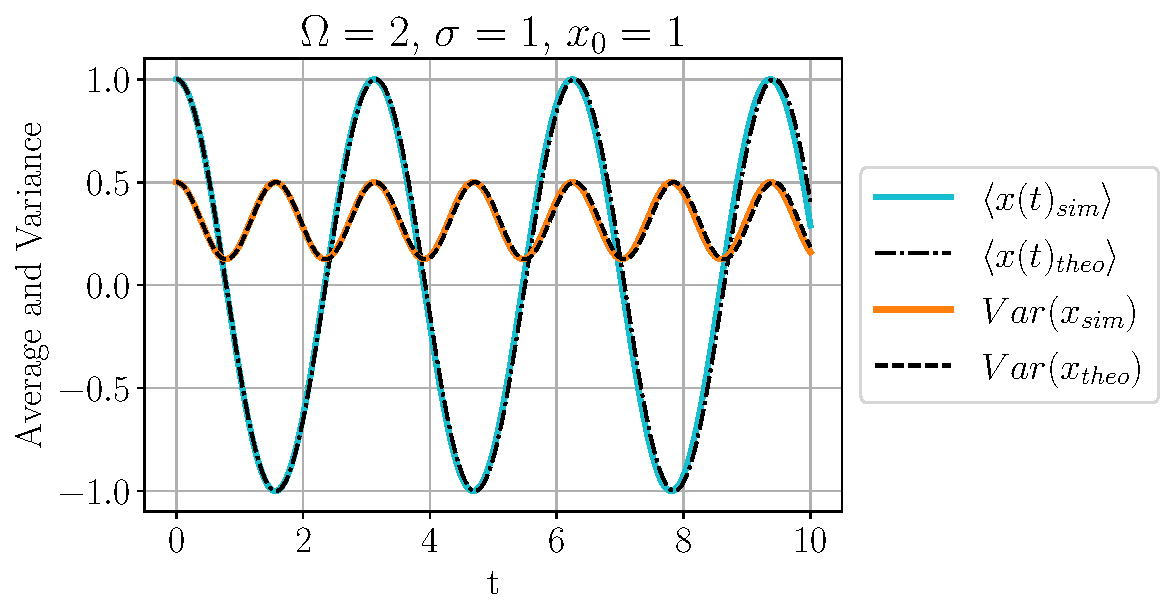
\includegraphics[width=\textwidth]{plot/Omega2_sigma1_x01_Averages.pdf}
         \caption{}
     \end{subfigure}
     \begin{subfigure}[h]{0.65\textwidth}
         \centering
         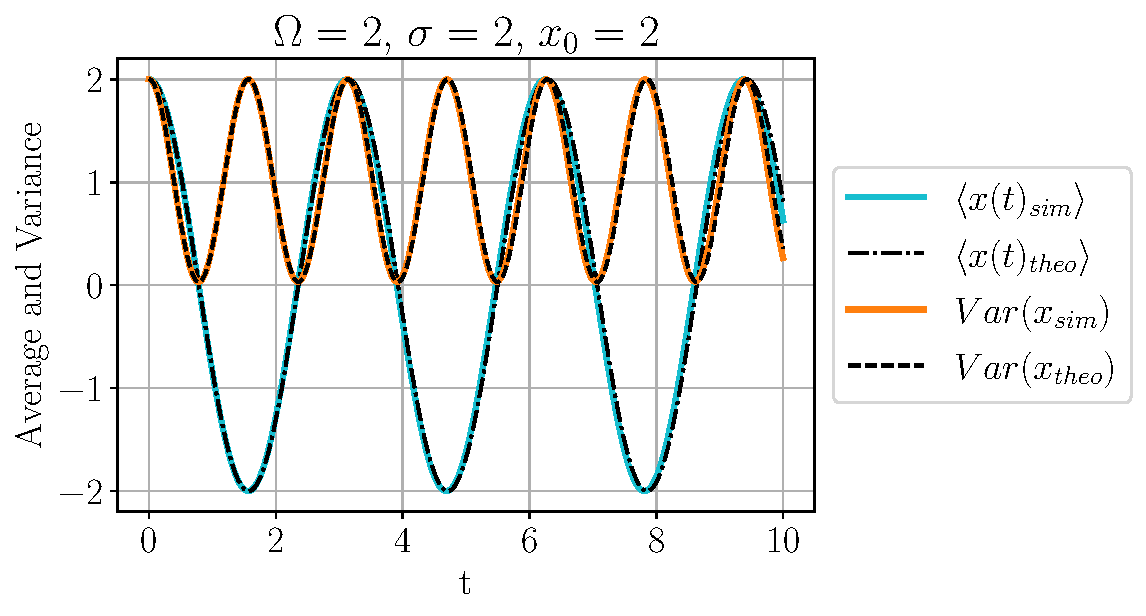
\includegraphics[width=\textwidth]{plot/Omega2_sigma2_x02_Averages.pdf}
         \caption{}
     \end{subfigure}
\caption{Simulation results for the average and variances for the position. In the title of each plot, the parameters $\Omega, \sigma$, and $x_0$ used are specified. The solid lines show the results according to the simulation model and the dashed line the theoretical expectation according to \refEq{eq: x sol} and \refEq{eq: xx sol}.}
\label{fig: Averages}
\end{figure}

\begin{figure}[h!]
     \begin{subfigure}[h]{0.65\textwidth}
         \centering
         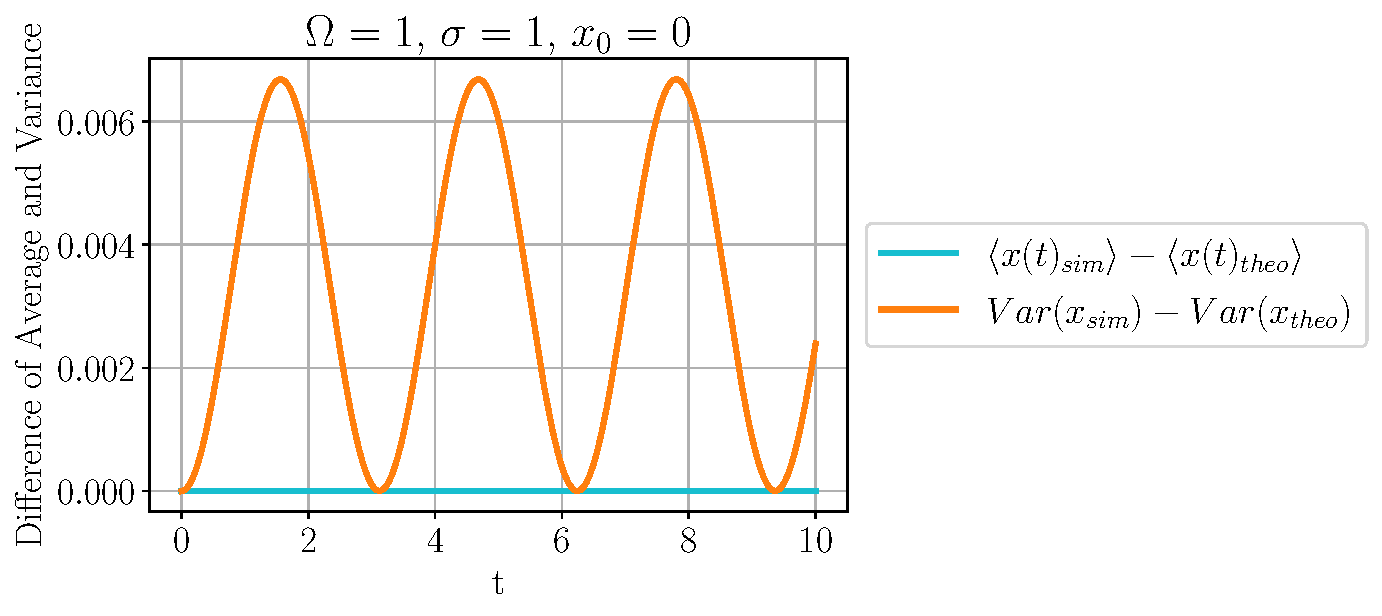
\includegraphics[width=\textwidth]{plot/Omega1_sigma1_x00_Averages_expect.pdf}
         \caption{}
         
     \end{subfigure}
     \begin{subfigure}[h]{0.4\textwidth}
         \centering
         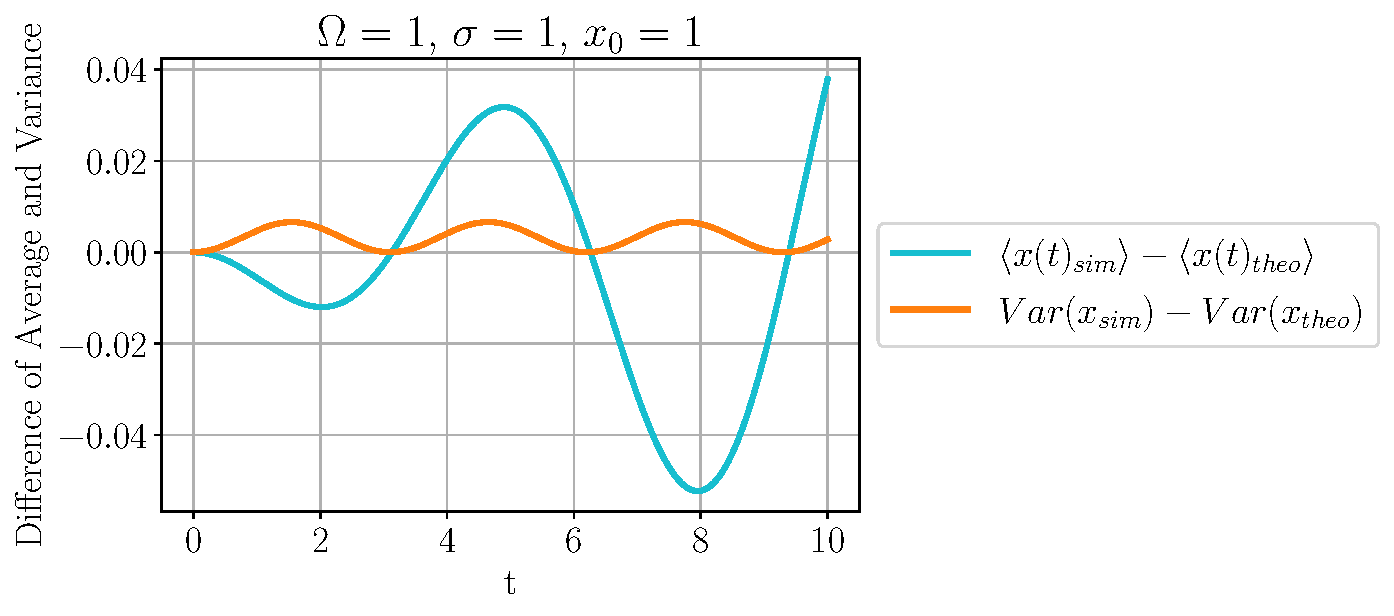
\includegraphics[width=\textwidth]{plot/Omega1_sigma1_x01_Averages_expect.pdf}
         \caption{}
         
     \end{subfigure}
     \begin{subfigure}[h]{0.65\textwidth}
         \centering
         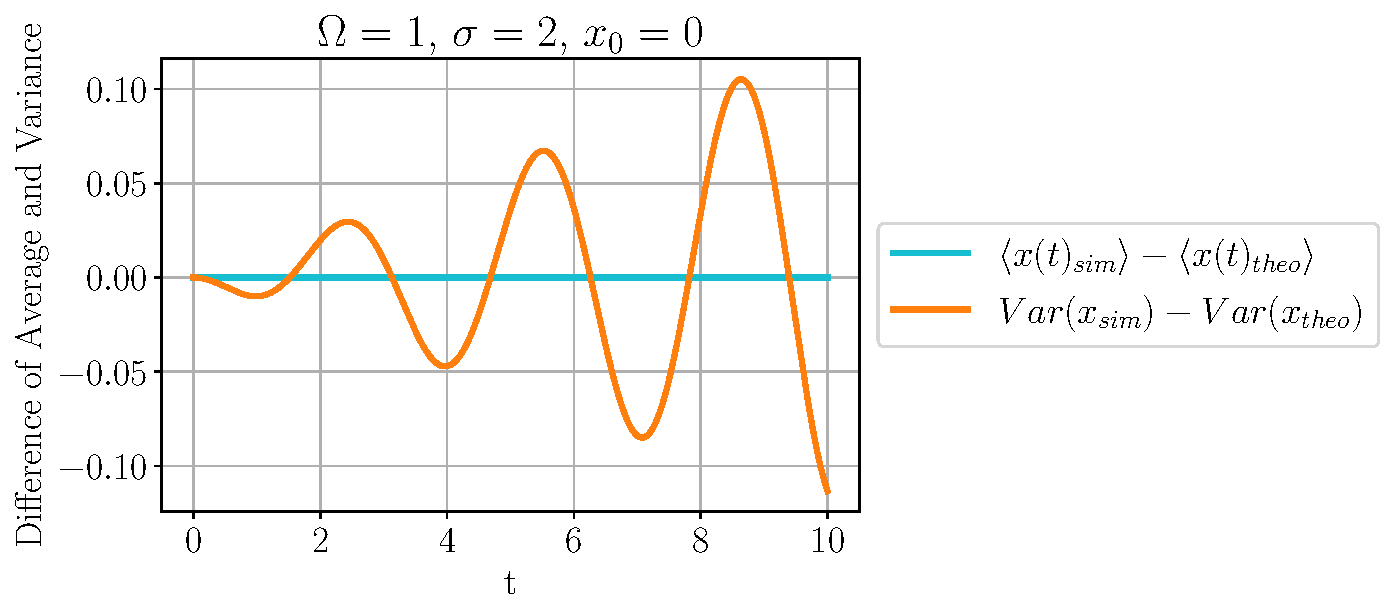
\includegraphics[width=\textwidth]{plot/Omega1_sigma2_x00_Averages_expect.pdf}
         \caption{}
         
     \end{subfigure}
     \begin{subfigure}[h]{0.4\textwidth}
         \centering
         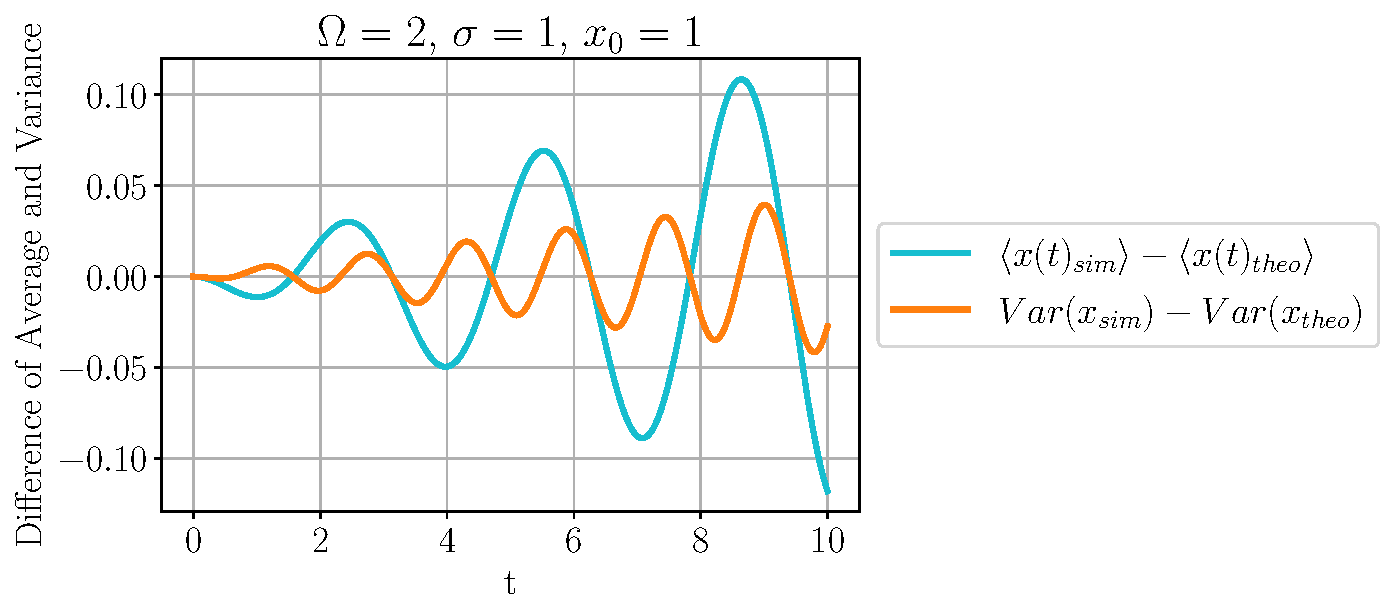
\includegraphics[width=\textwidth]{plot/Omega2_sigma1_x01_Averages_expect.pdf}
         \caption{}
     \end{subfigure}
     \begin{subfigure}[h]{0.65\textwidth}
         \centering
         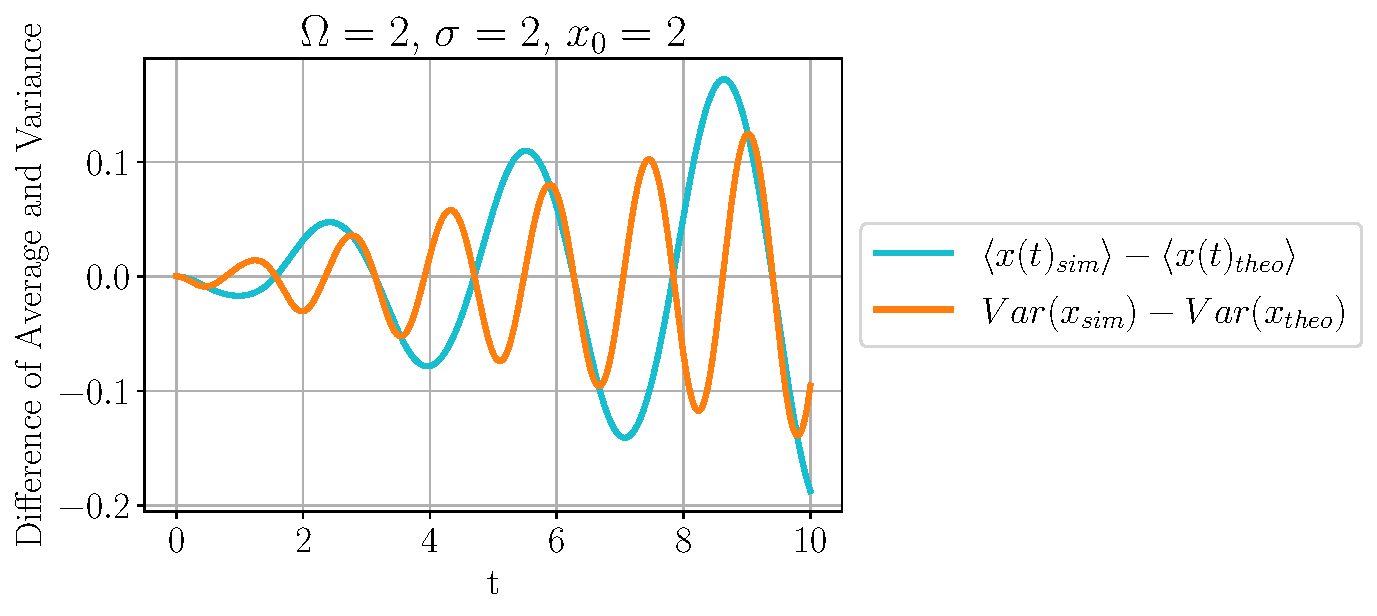
\includegraphics[width=\textwidth]{plot/Omega2_sigma2_x02_Averages_expect.pdf}
         \caption{}
     \end{subfigure}
\caption{Difference between simulation results and theoretical expectation for the average and variances for the position. In the title of each plot, the parameters $\Omega, \sigma$, and $x_0$ used are specified.}
\label{fig: difference}
\end{figure}



\begin{figure}[h!]
\centering
     \begin{subfigure}[h]{0.7\textwidth}
         \centering
         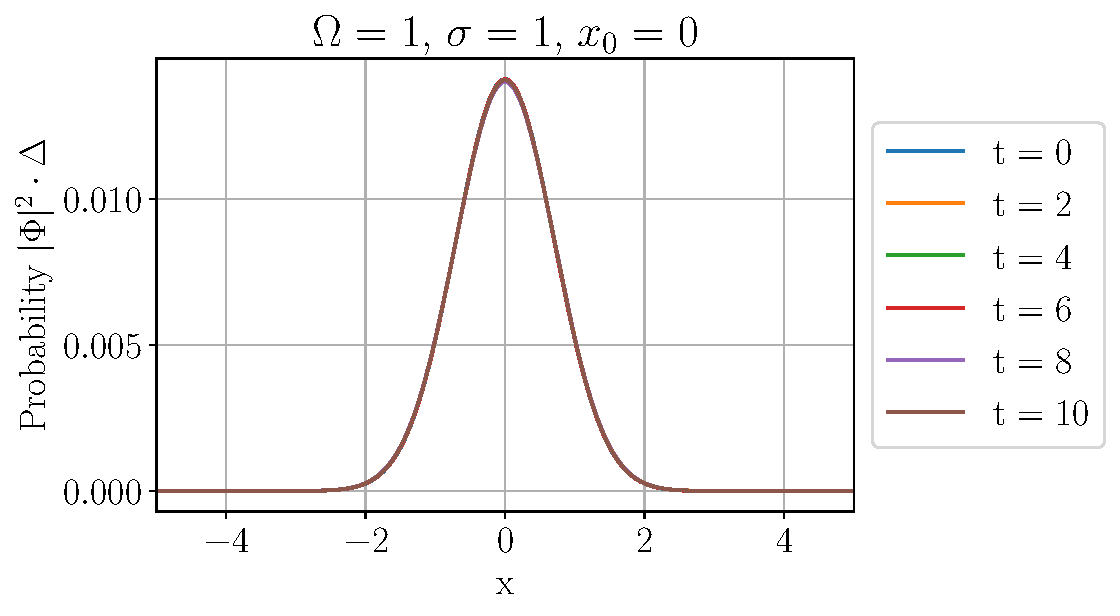
\includegraphics[width=\textwidth]{plot/Omega1_sigma1_x00_Probabilities.pdf}
         \caption{}
     \end{subfigure}

     \begin{subfigure}[h]{0.7\textwidth}
         \centering
         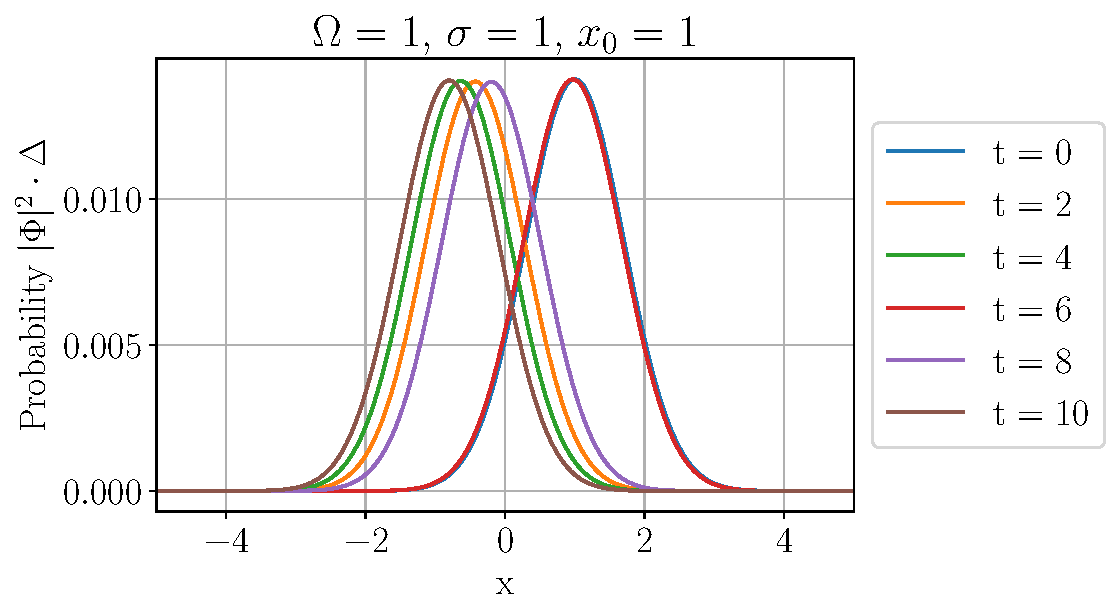
\includegraphics[width=\textwidth]{plot/Omega1_sigma1_x01_Probabilities.pdf}
         \caption{}
         
     \end{subfigure}
     
     \begin{subfigure}[h]{0.7\textwidth}
         \centering
         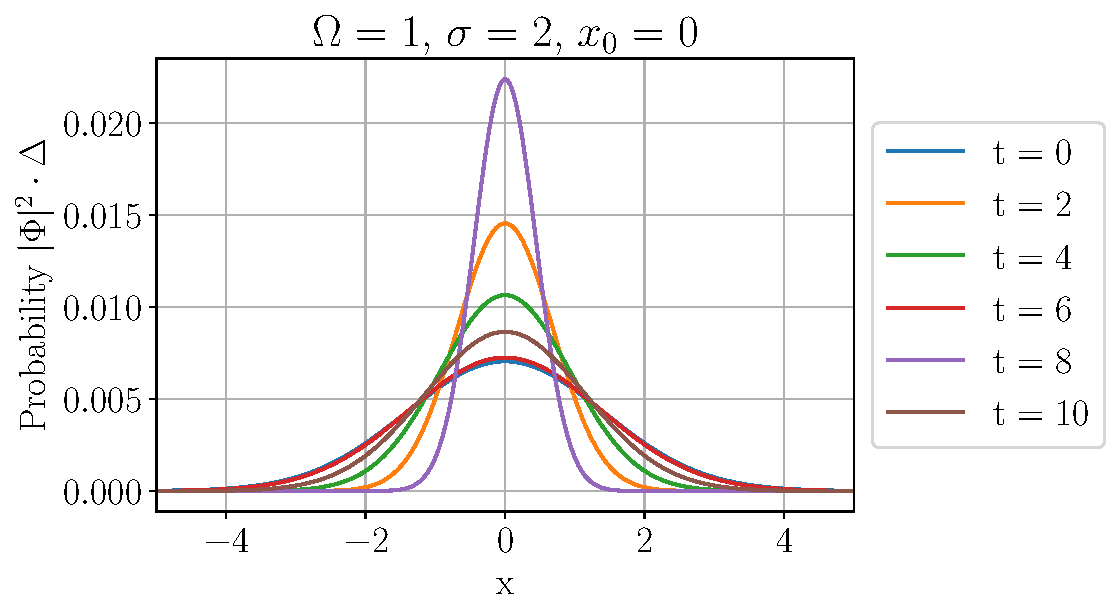
\includegraphics[width=\textwidth]{plot/Omega1_sigma2_x00_Probabilities.pdf}
         \caption{}
        
     \end{subfigure}
\end{figure}

\begin{figure}[h!]\ContinuedFloat
\centering
     \begin{subfigure}[h]{0.7\textwidth}
         \centering
         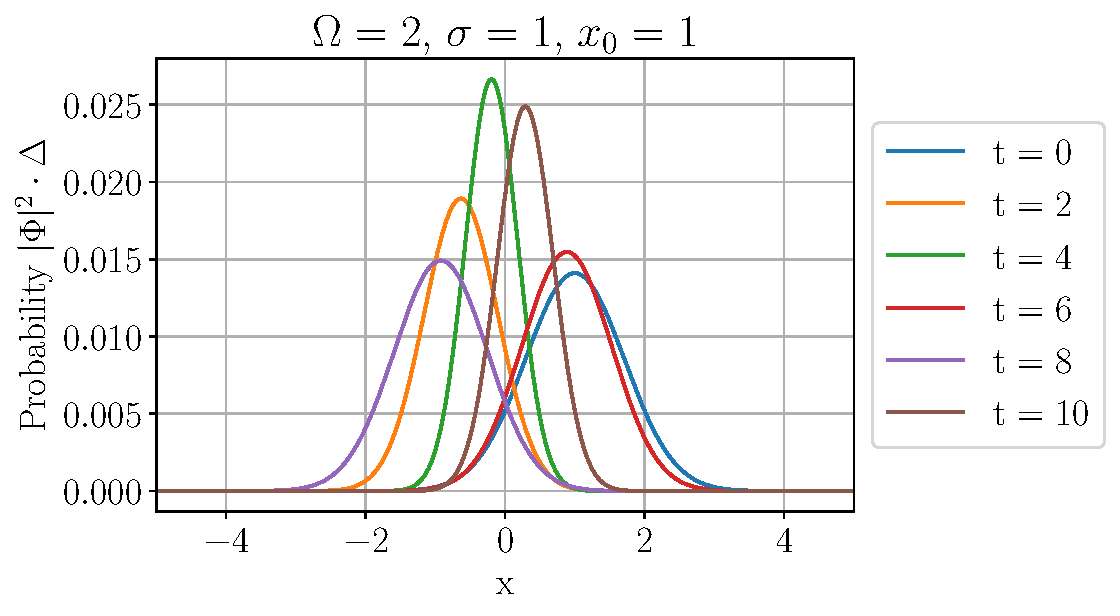
\includegraphics[width=\textwidth]{plot/Omega2_sigma1_x01_Probabilities.pdf}
         \caption{}
         
     \end{subfigure}
     
     \begin{subfigure}[h]{1\textwidth}
         \centering
         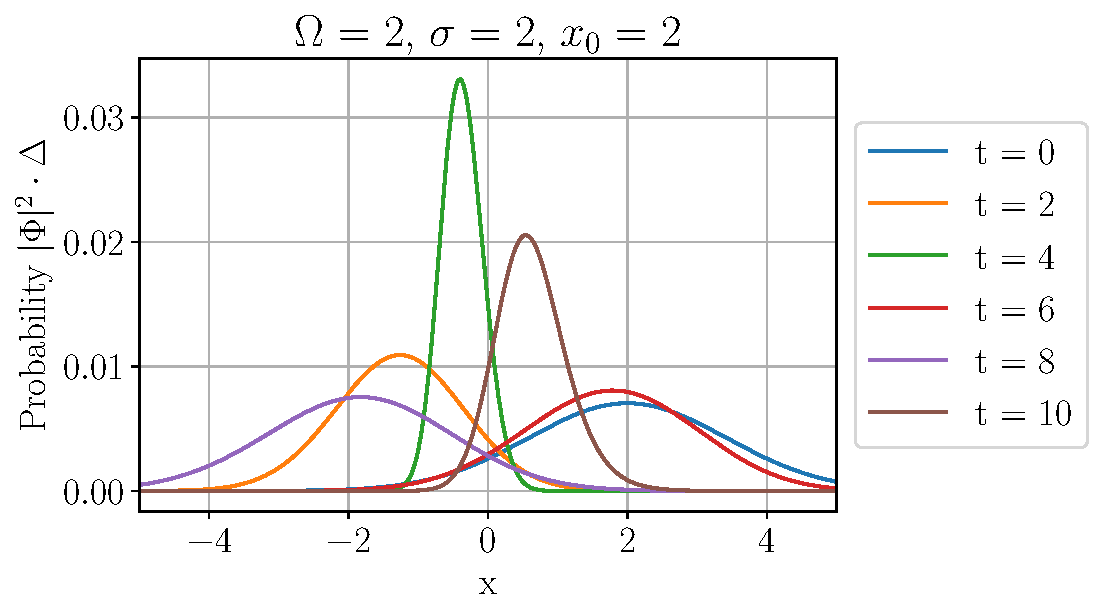
\includegraphics[width=\textwidth]{plot/Omega2_sigma2_x02_Probabilities.pdf}
         \caption{}
         
     \end{subfigure}
\caption{Simulation results for the Probabilities $|\Phi(x,t)|^2$. In the title of each plot, the parameters $\Omega, \sigma$, and $x_0$ used are specified. The functions are plotted for the six different times $t= 0,2,4,6,8,10$. The system is bounded to $-15 \leq x \leq 15$, but only $-5$ to $5$ is shown here.}
\label{fig: Probabilities}
\end{figure}

